\subsection*{1.1}
%1. Build the circuit shown below using BS170 transistor and a resistor RD = 470 . %Supply
%voltage is VDD = +15 V. Transistor gate is connected to a variable power supply.   
The circuit was built. The resistor, $R_D$, that is defined $470 \Omega$  is measured as $462 \Omega$.

    %FIG1 CIRCUIT DIAGRAM OF A HALFWAVE RECTIFIER
    \begin{figure}[h!]
        \centering
        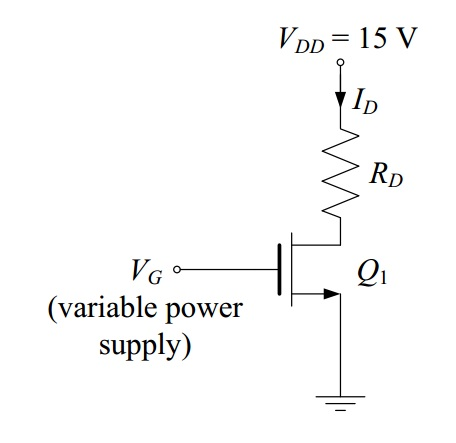
\includegraphics[width=6cm]{circuit_task_1.jpg}
        \captionof{figure}{The circuit in Task 1}
    \end{figure}

\subsection*{1.2}
% 2. Determine the threshold voltage and the transconductance parameter k of the MOS
%transistor. 
%In particular, find the voltage VT for which noticeable drain current appears,
The threshold voltage is determined by observing the drain current whilst increasing the voltage at the gate. When the current is significantly large compared to zero the threshold voltage is the voltage at that point. Therefore: $$V_T = 1.9 \ V$$.

The transconductance factor can be estimated by taking one point from the graph when $V_G > V_T$. The point chosen was $I_{D_0} \approx 10 \ mA = 9.255 \ mA $ and corresponding gate voltage is $V_{G_0} = 2.1 \ V$. Therefore: $$ k = \dfrac{I_{D_0}}{(V_{G_0}-V_T)^2} = \dfrac{9.255 \ mA}{(2.1 \ V - 1.9 \ V)^2} = 231.14 \ \dfrac{mA}{V^2} $$

\begin{figure}[h!]
        \centering
        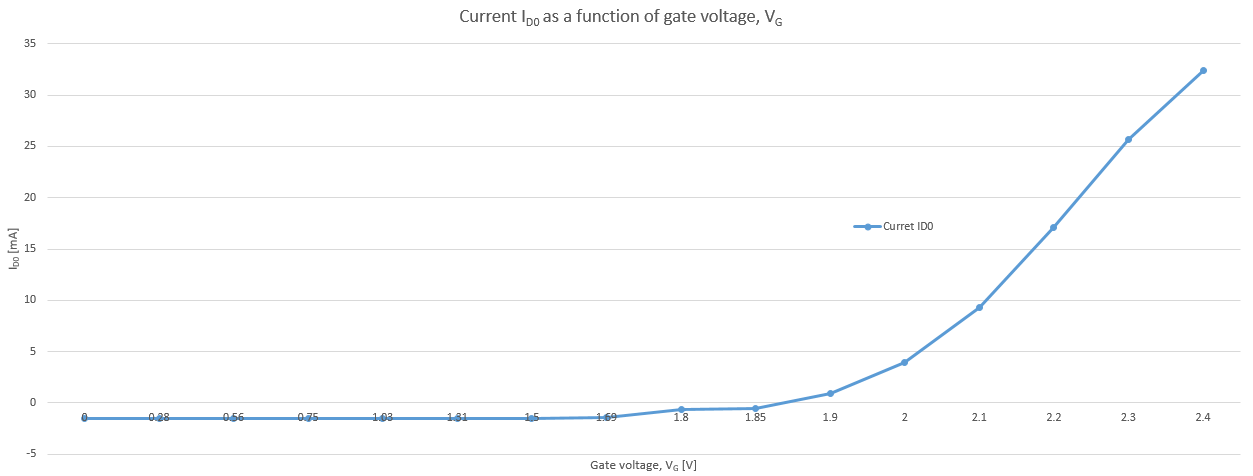
\includegraphics[width=16cm]{Task1.png}
        \captionof{figure}{Plot of the drain current versus the gate voltage ($I_D$ vs. $V_G$)}
\end{figure}

%Note that the parameter k here includes W/L and 0.5 factor
%that you have in the drain current formula ID = 0.5 kn’W/L(VGS–VT)2, i.e., k = 0.5kn’W/L.






